\documentclass[10pt]{beamer}

\input{/Users/daniel/Documents/LaTeX/beamer-style.tex}


\title{Développement d'applications mobiles}
\subtitle{Chapitre 2 - Dart - concepts de base}
\date{\today}
\author{Daniel Schreurs}
\institute{Haute École de la Province de Liège}
%\titlegraphic{\hfill\includegraphics[height=1.5cm]{logo.eps}}

\begin{document}

\maketitle

\setbeamerfont{subsection in toc}{size=\small}
\begin{frame}[allowframebreaks]{Table des matières}
    \setbeamertemplate{section in toc}[sections numbered]
    \tableofcontents
\end{frame}

\section{Dart}
\subsection{Présentation}
\begin{frame}[fragile,t]{\secname : \subsecname}
    \begin{itemize}
        \item Deux développeurs de Google : Lars Bak et Kasper Lund (2010);
        \item Version 1.0 : 2011;
        \item Adopté par ECMA International en 2014;
        \item Version 2.0. 2018.
    \end{itemize}
\end{frame}

\subsection{DartPad}
\begin{frame}[fragile,t]{\secname : \subsecname}
    \begin{itemize}
        \item Éditeur entièrement en ligne et gratuit;
        \item Permet d'isoler une problématique à la fois.
    \end{itemize}
    \begin{figure}
        \begin{center}
            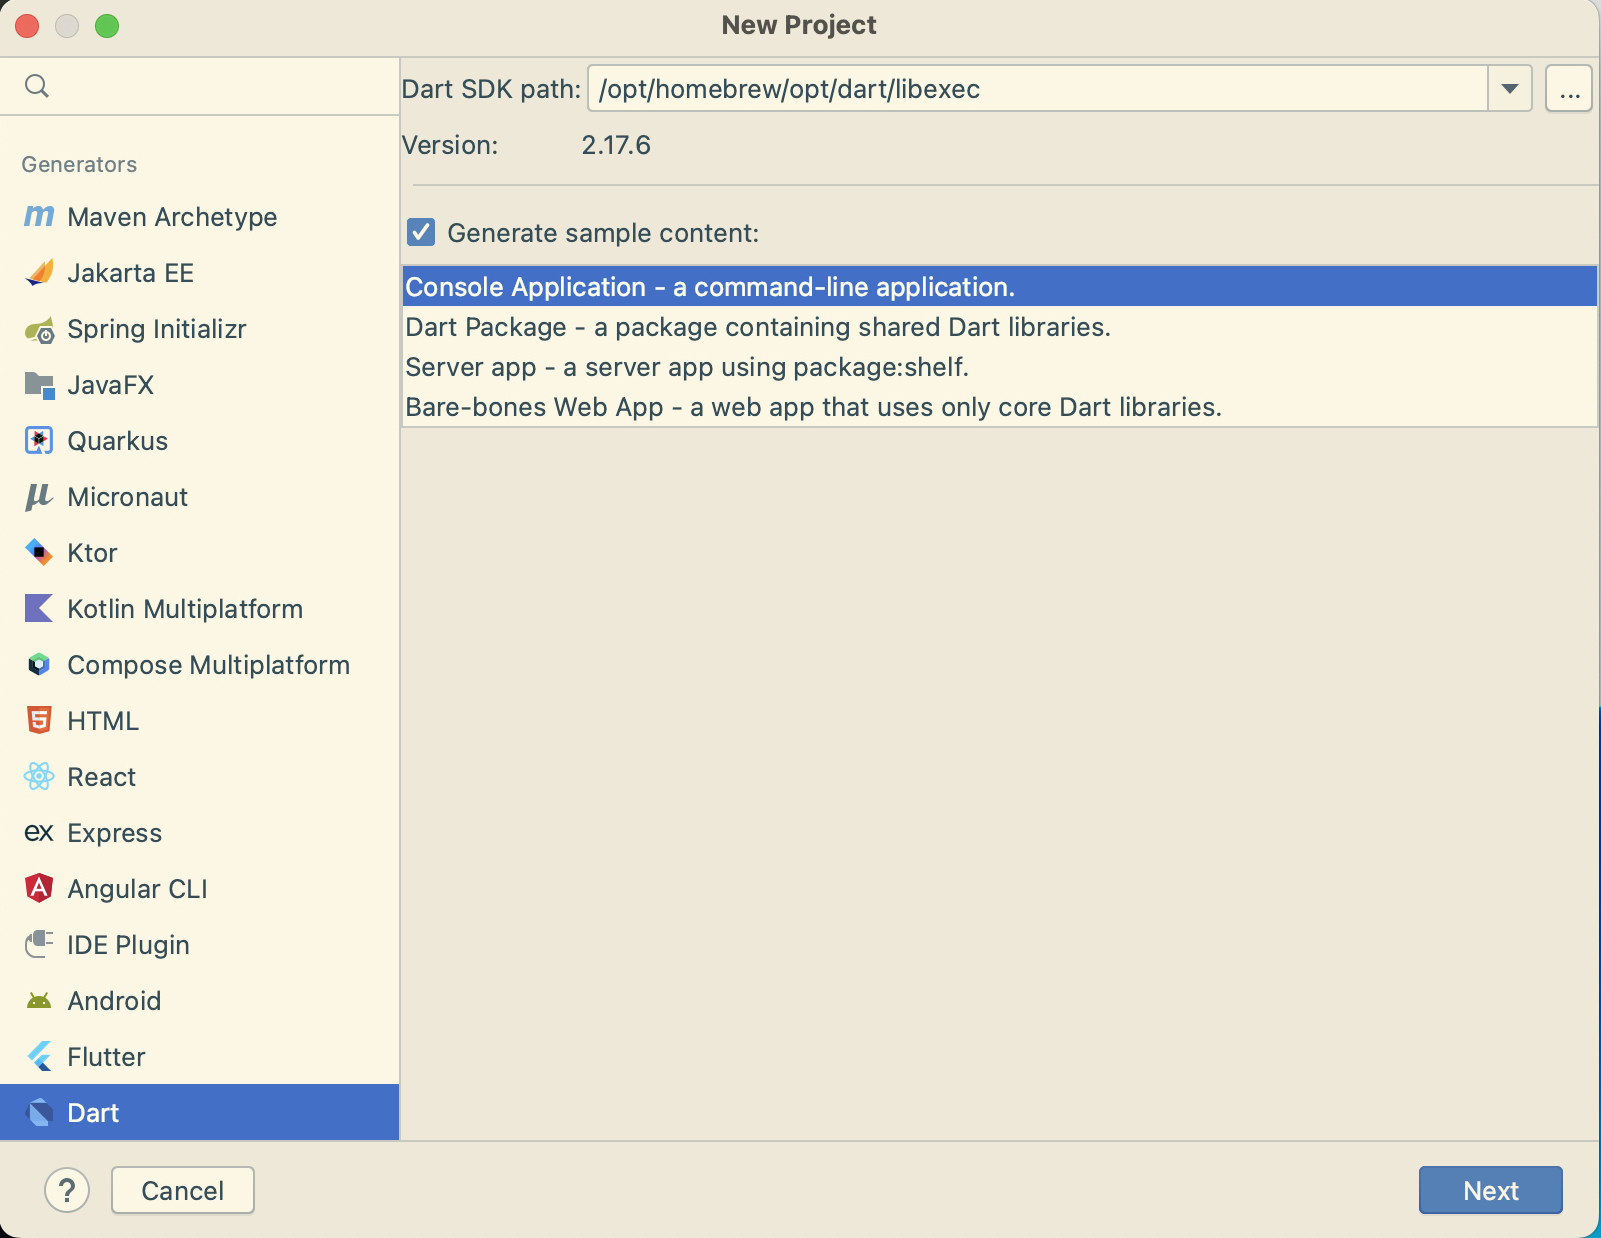
\includegraphics[width=0.60\textwidth]{../assets/img/new-project-1--dart.jpg}
            \caption*{Nouveau projet console - Dart}
        \end{center}
    \end{figure}
\end{frame}

\section{Variables}
\subsection{Les nombres}
\begin{frame}[fragile,t]{\secname : \subsecname}
    \begin{itemize}
        \item Les entiers (Integer);
        \item les nombres réels (Double).
    \end{itemize}
    \begin{lstlisting}[language={c}]
        int monEntier; 
        double monReel;
    \end{lstlisting}
    \begin{alertblock}{Important}
        Si la variable n’est pas initialisée avec une valeur choisie, elle prendra \lstinline[language=c]!null! comme valeur par défaut.
    \end{alertblock}
\end{frame}

\subsection{Les chaines de caractères}
\begin{frame}[fragile,t]{\secname : \subsecname}
    \begin{itemize}
        \item La déclaration et l’initialisation des chaines de caractères sont semblables à celle des nombres;
        \item La valeur de la chaine est entourée de simples ou doubles guillemets;
        \item Conversion depuis un nombre (ou autre) grâce à la fonction \lstinline[language=sql]!toString()!;
        \item Une chaine de caractères est un objet, on peut appeler d'autres méthodes \lstinline[language=sql]!toLowerCase()!.
    \end{itemize}
    \lstinputlisting[language=java]{../exemples/Chapitre 2 - Dart - concepts de base/chapitre-2-dart-concepts-de-base/bin/string.dart}
\end{frame}

\subsection{Les booléens}
\begin{frame}[fragile,t]{\secname : \subsecname}
    \begin{itemize}
        \item Un autre type très courant;
        \item extrêmement utile;
        \item valeurs vrai ou faux.
    \end{itemize}
    \lstinputlisting[language=java]{../exemples/Chapitre 2 - Dart - concepts de base/chapitre-2-dart-concepts-de-base/bin/bool.dart}
\end{frame}

\subsection{Le type var}
\begin{frame}[fragile,t]{\secname : \subsecname}
    \begin{itemize}
        \item Utilisés quand on ne souhaite pas typer une variable au moment de sa déclaration;
        \item Au \textit{runtime}, le système déterminera le type approprié;
        \item Une fois déterminé, plus possible de changer.
    \end{itemize}
    \lstinputlisting[language=java]{../exemples/Chapitre 2 - Dart - concepts de base/chapitre-2-dart-concepts-de-base/bin/bool.dart}
\end{frame}

\subsection{Le type Dynamic}
\begin{frame}[fragile,t]{\secname : \subsecname}
    \begin{itemize}
        \item Utilisés quand on ne souhaite pas typer une variable;
        \item Au \textit{runtime}, le système déterminera à chaque affectation le type approprié;
        \item Une fois déterminé, le type peut changer.
    \end{itemize}
    \lstinputlisting[language=java]{../exemples/Chapitre 2 - Dart - concepts de base/chapitre-2-dart-concepts-de-base/bin/dynamic.dart}
\end{frame}

\section{Constantes}
\subsection{final}
\begin{frame}[fragile,t]{\secname : \subsecname}
    \begin{itemize}
        \item Rend une valeur affectée immuable;
        \item Elle ne pourra plus être changée;
        \item C'est la référence vers la valeur qui ne peut pas changer.
    \end{itemize}
    \lstinputlisting[language=java]{../exemples/Chapitre 2 - Dart - concepts de base/chapitre-2-dart-concepts-de-base/bin/final.dart}
\end{frame}
\subsection{const}
\begin{frame}[fragile,t]{\secname : \subsecname}
    \begin{itemize}
        \item Encore plus restrictif;
        \item La valeur doit être connue au moment de la déclaration.
    \end{itemize}
    \lstinputlisting[language=java]{../exemples/Chapitre 2 - Dart - concepts de base/chapitre-2-dart-concepts-de-base/bin/final.dart}
\end{frame}

\section{Collections}
\subsection{Listes}
\begin{frame}[fragile,t]{\secname : \subsecname}
    \begin{itemize}
        \item Les listes permettent de définir une collection;
        \item Chaque item est associé à un index qui démarre à partir de 0;
        \item Voir \href{https://dart.dev/null-safety}{null safety} pour les tableaux vides;
        \item Une liste sera de taille fixe ou modulaire.
    \end{itemize}
    \lstinputlisting[language=java]{../exemples/Chapitre 2 - Dart - concepts de base/chapitre-2-dart-concepts-de-base/bin/list.dart}
\end{frame}

\subsection{Maps}
\begin{frame}[fragile,t]{\secname : \subsecname}
    \begin{itemize}
        \item Type de collection;
        \item Système de couple clé/valeur.
    \end{itemize}
    \lstinputlisting[language=java]{../exemples/Chapitre 2 - Dart - concepts de base/chapitre-2-dart-concepts-de-base/bin/maps.dart}
\end{frame}

\section{Structures de contrôle}
\begin{frame}[fragile,t]{\secname}
    Toutes les structures de contrôle habituelles sont présentent :
    \begin{itemize}
        \item Les tests : \lstinline[language=sql]!if!,\lstinline[language=sql]!else!, \lstinline[language=sql]!else if!, \lstinline[language=sql]!Switch!;
        \item L'opérateur ternaire : \lstinline[language=sql]!?:!;
        \item les boucles : \lstinline[language=sql]!for!,\lstinline[language=sql]!Foreach!,\lstinline[language=sql]!While!,\lstinline[language=sql]!Do While!
    \end{itemize}
\end{frame}

\section{Les fonctions}
\subsection{Paramètres optionnels}
\begin{frame}[fragile,t]{\secname : \subsecname}
    \begin{itemize}
        \item La fonction \lstinline[language=sql]!main! => point d’entrée du programme;
        \item les fonctions peuvent retourner des valeurs;
        \item les fonctions peuvent prendre des paramètres;
        \item les fonctions peuvent prendre des paramètres optionnels.
    \end{itemize}
    \lstinputlisting[language=java]{../exemples/Chapitre 2 - Dart - concepts de base/chapitre-2-dart-concepts-de-base/bin/function.dart}
\end{frame}

\subsection{anonymes}
\begin{frame}[fragile,t]{\secname : \subsecname}
    \begin{itemize}
        \item Inscrites dans le code pour un besoin unique;
        \item Ne pourront pas être appelées à un autre endroit.
    \end{itemize}
    \lstinputlisting[language=java]{../exemples/Chapitre 2 - Dart - concepts de base/chapitre-2-dart-concepts-de-base/bin/anonymes.dart}
\end{frame}

\subsection{fléchées}
\begin{frame}[fragile,t]{\secname : \subsecname}
    \begin{itemize}
        \item Comme les fonctions anonymes;
        \item Syntaxe est plus courte;
        \item Une seule ligne de code;
        \item \lstinline[language=sql]!return! implicit.
    \end{itemize}
    \lstinputlisting[language=java]{../exemples/Chapitre 2 - Dart - concepts de base/chapitre-2-dart-concepts-de-base/bin/arrow-function.dart}
\end{frame}

\section{Les classes}
\subsection{déclaration}
\begin{frame}[fragile,t]{\secname : \subsecname}
    \begin{itemize}
        \item Une classe par fichier (avec une majuscule);
        \item Pas de \lstinline[language=sql]!private! à la place un \lstinline[language=sql]!_!;
        \item les \lstinline[language=sql]![]! rendent un paramètre optionnel;
        \item On peut nommer des constructeurs \lstinline[language=sql]!NomDeLaClasse.NomConstructeur!;
        \item On peut surcharger les méthodes héritées.
    \end{itemize}
\end{frame}
\begin{frame}[fragile,t]{\secname : \subsecname}
    \lstinputlisting[language=java]{../exemples/Chapitre 2 - Dart - concepts de base/chapitre-2-dart-concepts-de-base/bin/class-dec.dart}
\end{frame}

\subsection{instanciation}
\begin{frame}[fragile,t]{\secname : \subsecname}
    \lstinputlisting[language=java]{../exemples/Chapitre 2 - Dart - concepts de base/chapitre-2-dart-concepts-de-base/bin/class-init.dart}
\end{frame}

\subsection{Accesseurs et mutateurs (getters et setters)}
\begin{frame}[fragile,t]{\secname : \subsecname}
    \lstinputlisting[language=java]{../exemples/Chapitre 2 - Dart - concepts de base/chapitre-2-dart-concepts-de-base/bin/class-set-get.dart}
\end{frame}

\subsection{Héritage}
\begin{frame}[fragile,t]{\secname : \subsecname}
    \begin{alertblock}{Important}
        Pas l’héritage multiple.
    \end{alertblock}
    \lstinputlisting[language=java]{../exemples/Chapitre 2 - Dart - concepts de base/chapitre-2-dart-concepts-de-base/bin/class-herit.dart}
\end{frame}

\subsection{Interface (classe abstraite)}
\begin{frame}[fragile,t]{\secname : \subsecname}
    \begin{alertblock}{Important}
        Le mot-clé \lstinline[language=sql]!Interface! n'existe pas.
    \end{alertblock}
    \lstinputlisting[language=java]{../exemples/Chapitre 2 - Dart - concepts de base/chapitre-2-dart-concepts-de-base/bin/interface.dart}
\end{frame}

\subsection{Mixin - inclure une autre classe}
\begin{frame}[fragile,t]{\secname : \subsecname}
    \lstinputlisting[language=java]{../exemples/Chapitre 2 - Dart - concepts de base/chapitre-2-dart-concepts-de-base/bin/class-mixin.dart}
\end{frame}

\section{Les exceptions}
\subsection{Structure}
\begin{frame}[fragile,t]{\secname : \subsecname}
    \lstinputlisting[language=java]{../exemples/Chapitre 2 - Dart - concepts de base/chapitre-2-dart-concepts-de-base/bin/try.dart}
\end{frame}

\subsection{exceptions système}
\begin{frame}[fragile,t]{\secname : \subsecname}
    \begin{itemize}
        \item \lstinline[language=sql]!DefferredLoadException! : levée quand une bibliothèque différée ne se charge pas;
        \item \lstinline[language=sql]!FormatException! : levée lorsqu’une chaine de caractères ou d’autres données ne possèdent
              pas le format attendu et ne peuvent pas être converties ou traitées;
        \item \lstinline[language=sql]!IntegerDivisionByZeroException! : levée quand une division par zéro est tentée sur un nombre;
        \item \lstinline[language=sql]!IOException! : levée quand un problème survient lors des opérations de types IO (Input/Output);
        \item \lstinline[language=sql]!IsolateSpawnException! : levée quand un isolate ne peut pas être créé;
        \item \lstinline[language=sql]!TimeOutException! : levée lorsqu’un délai d’expiration planifié est atteint en attendant un résultat asynchrone.
    \end{itemize}
\end{frame}

\subsection{Exceptions personnalisées}
\begin{frame}[fragile,t]{\secname : \subsecname}
    \lstinputlisting[language=java]{../exemples/Chapitre 2 - Dart - concepts de base/chapitre-2-dart-concepts-de-base/bin/ExceptionPerso.dart}
\end{frame}


\section{Traitement asynchrone}
\subsection{async et await}
\begin{frame}[fragile,t]{\secname : \subsecname}
    \begin{itemize}
        \item L’asynchronicité est la possibilité pour une tâche d’être réalisée en parallèle d’une autre dans un laps de temps qui diffère.
        \item Éviter de bloquer l’application;
        \item Le reste du programme doit continuer;
        \item Par exemple, obtenir de l’information depuis une base de données.

    \end{itemize}
    \begin{alertblock}{Important}
        Deux mots-clés :\lstinline[language=sql]!async! et \lstinline[language=sql]!await!.
    \end{alertblock}
\end{frame}

\subsection{Future<T>}
\begin{frame}[fragile,t]{\secname : \subsecname}
    \begin{itemize}
        \item Disponible dans le \emph{futur}.
        \item Représenter une réussite ou un échec :
              \begin{itemize}
                  \item Résultat d’un calcul;
                  \item Récupération de données, etc.
              \end{itemize}
    \end{itemize}
\end{frame}

\begin{frame}[fragile,t]{\secname : \subsecname}
    \lstinputlisting[language=java]{../exemples/Chapitre 2 - Dart - concepts de base/chapitre-2-dart-concepts-de-base/bin/future.dart}
\end{frame}



\end{document}